\documentclass[7pt]{article}
\usepackage{graphicx}
\usepackage{float}
\usepackage{amsmath}
\usepackage{amsfonts}
\usepackage{multicol}
\usepackage{pdfpages}
\usepackage[backend=biber]{biblatex}
\bibliography{report.bib}
\usepackage[bindingoffset=0.0in,%
            left=0.9in,right=0.9in,top=1.0in,bottom=0.8in,%
            voffset=0in,footskip=1.5in]{geometry}
\usepackage{titling}


%\setlength{\intextsep}{1.5pt}
%\setlength{\textfloatsep}{-1in}

\begin{document}

%\newgeometry{margin=1in}

\begin{titlepage}
	\centering
	{\scshape\Large \par}
	\vspace{3.5cm}
	{\huge\bfseries A theoretical framework for Attention\par}
	\vspace{1cm}
	{\itshape Erik de Godoy Perillo\par}
	{\itshape Advisor: Profa. Dra. Esther Luna Colombini\par}
	\vspace{0.5cm}
	\vfill
	State University of Campinas
	\vfill
	{\large \today\par}
\end{titlepage}

\newpage



%\begin{multicols}{2}

\section{Introduction}
In this document, we briefly formulate a theoretical framework for the concept of Attention.
This framework consists of two main parts:
\begin{itemize}
    \item A \emph{definition} of Attention in terms of its functionalities;
    \item A \emph{model} of Attention.
\end{itemize}
Note that the first element aims at answering the question ``\emph{What} is Attention?''
while the second aims at explaining \emph{how} Attention emerges.

\section{A definition of Attention}
\label{sec:definition}
In this definition, we define a set of \emph{entities of interest} and the phenomenon of Attention in terms of
its \emph{functionalities} and how it relates to the entities.

\subsection{Why is our definition good?}
We believe our definition encompasses what we generally (and intuitively) refer to as attention while being not too broad.
Also, the definition is given in terms related to Computer Science so it’s functionality nicely translates to the domain,
which is important since we (so far) intend to develop AI using computers as we know it today.
We may not encompass every aspect of Attention and even be conflicting with other definitions.
However, this is the set of postulates that we think is the most precise and useful and thus this is
what we choose to use for future work to be based on.

\subsection{Entities}
Below is the list of entities - or ``terms'' - we use in this work, along with a brief discussion of the meaning
we give to each term in the context of this work.

\begin{itemize}
    \item\textbf{Data:} information, stimuli. It may be internal or external. Examples: visual information, audio, memories.
    \item\textbf{Program:} algorithm, sequence of computer (or mental) operations. Programs use data as input in order to carry out a sequence of operations that produces output data and/or actions.
    \item\textbf{Process:} the execution of a program on a specific data instance.
    \item\textbf{Computer:} the executor of processes, the “brain”.
    \item\textbf{Resource:} when not specified, we mean “computational resources”, e.g. CPU time.
    \item\textbf{Time:} the flow of time.
    \item\textbf{World:} the external environment.
    \item\textbf{Agent:} the actor in the world.
    \item\textbf{Actions:} the interaction of the agent with the world.
    \item\textbf{Goals:} the ends, objectives to be met.
\end{itemize}

\subsection{What is Attention?}
\emph{Data}, \emph{programs} and \emph{processes} are virtually \emph{infinite}.
Computational \emph{resources} and \emph{actions} are finite.
\emph{Attention} is \emph{the system of allocating resources to processes}.
In other words, \emph{attention} is the entity in \emph{agents} that, given \emph{context} and a set of \emph{processes},
\emph{allocates} \emph{resources} to execute each of them in order to \emph{produce} \emph{outputs} in form of \emph{data} and \emph{actions} in a \emph{correct sequential manner} and in \emph{sensible time} in order to reach \emph{goals}.

\section{A model of Attention}
We propose a model for the phenomenon of Attention.
Following the definition given in section~\ref{sec:definition}, in our model we assume that Attention takes place in the context
of a ``mind'' that behaves like a computer that executes processes: it processes inputs via algorithms to produce an output in discrete steps.
We propose that \emph{Attention can emerge in any process} to be executed by such mind by means of \emph{a series of components} -- which we call \emph{attentional modules}. These modules can alter data being processed and the execution flow of the algorithm and provide the functionalities of Attention.

\begin{figure}[H]
    \centering
    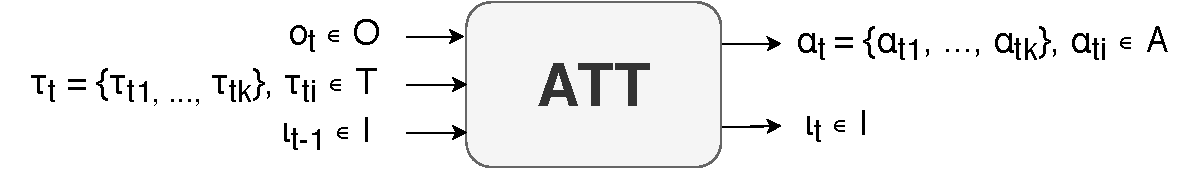
\includegraphics[width=0.9\linewidth]{./img/alt_att_block.pdf}
    \label{fig:attmodule}
    \caption{Attentional module.}
\end{figure}

Figure~\ref{fig:attmodule} illustrates the attentional module. At each time step $t$, the module receives as \emph{input}:
\begin{itemize}
    \item Current \emph{outer state} $o_t \in O$, where $O$ is the \emph{outer state set}.
    \item Group of \emph{focus targets} $\tau_t = \{\tau_{t1}, ..., \tau_{tk}\}, \tau_{ti} \in T$,
        where $T$ is the \emph{focus target set}.
    \item Past \emph{inner state} $\iota_{t-1} \in I$, where $I$ is the \emph{inner state set}.
\end{itemize}

The module produces as \emph{output} (as a function of both inputs):
\begin{itemize}
    \item Current \emph{inner state} $\iota_t \in I$.
    \item Current \emph{focus output} $\alpha_t = \{\alpha_{t1}, ..., \alpha_{tk}\}, \alpha_{ti} \in A$,
        where $A$ is the \emph{focus output set}.
\end{itemize}

\subsection{Focus output}
The focus output is the main element of the module: it can be used to allocate \emph{finite resources} to a set of ``candidate targets'' by giving them an ``importance score'' which can be used in any arbitrary way in following steps -- such as choosing the amount of computation to be dedicated to an element or which elements will be used as input to another step.
Each element $\alpha_{tk}$ is respective to a target element $\tau_{tk}$.
Target elements ($\tau \in T$) may effectively be \emph{programs} (tasks) or \emph{data}.

\subsubsection{Soft and Hard Attention}
The focus output will generally be such that it acts as either \emph{Soft} or \emph{Hard Attention}:
\begin{itemize}
    \item \textbf{Soft Attention:}
        $A = [0, 1]$, with $0 \le \sum_{i=1}^{k} \alpha_{ti} \le 1$
    \item \textbf{Hard Attention:}
        $A = \{0, 1\}$, with $0 \le \sum_{i=1}^{k} \alpha_{ti} \le M$ and $0 \le M \le |\tau_t|$
\end{itemize}

\subsubsection{Using the output of the focus function}
The focus function output may be used for the allocation of some resource in various ways, such as:
\begin{itemize}
    \item Choosing the \textbf{amount} of \textbf{computation time} to be used at a certain step;
    \item Choosing a \textbf{subset} of \textbf{elements} to carry out further computations;
    \item \textbf{Weighting elements} to perform a certain computation.
\end{itemize}

\subsection{Modules forming an attentional system}
A system with Attention may contain more than one attentional modules -- even in a recursive manner.
Together, these modules always perform the function to allocate resources to
processes.

Figure~\ref{fig:attsystem} shows the diagram of a possible system with attention.
The module \emph{TaskATT} uses hard attention to select a certain task $k$ to be executed for some time at time step $t$.
Among the computations of task $k$, there is the module \emph{DataATT}, uses soft attention to allocate resources to a set of items.
It is worth noting that time is relative to each attentional module: \emph{TaskATT} has a temporal course over time steps $t$ that is different from that of \emph{DataATT}, which is over time steps $t'$.
Also, their sets of inputs and outputs may differ.

\begin{figure}[H]
    \centering
    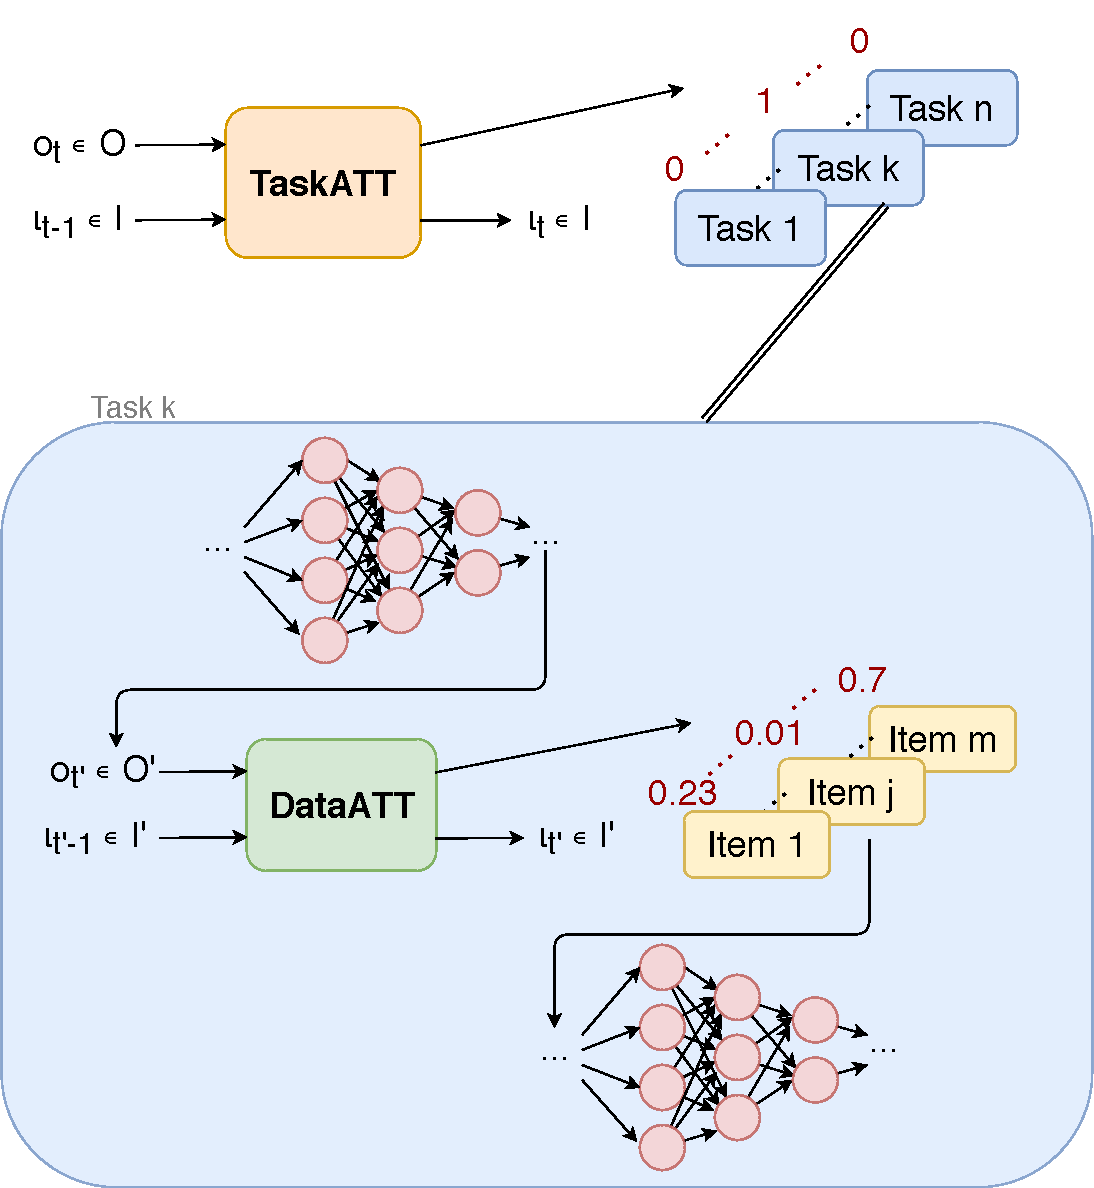
\includegraphics[width=0.7\linewidth]{./img/att_blocks_example.pdf}
    \label{fig:attsystem}
    \caption{Example of a system that uses attention.}
\end{figure}

\section{Validating the framework}
In this section, we investigate some recent works on attention and see how they fit in our framework.

\subsection{Image Caption Generation}
The work~\cite{ref:show-attend-tell} is among the first to propose using
attention to image caption generation: the encoding of the input image is
represented as a set of vectors -- each respective to a certain spatial region of the image --
and the attentional component gives weights to each vector at each step in order to produce another
vector to be used in further computations.

\begin{figure}[H]
    \centering
    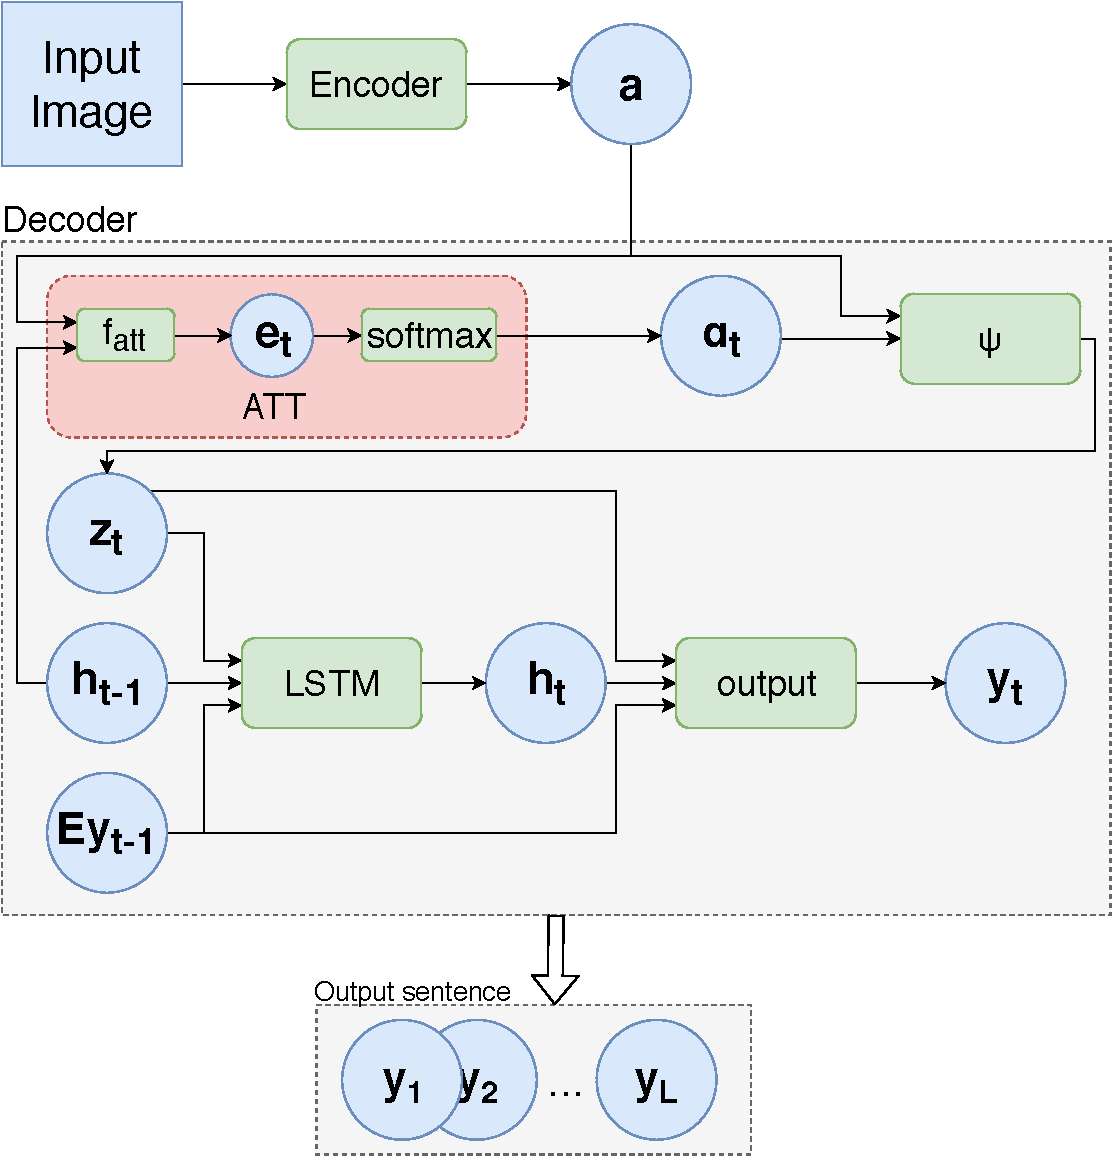
\includegraphics[width=0.6\linewidth]{./img/captioning.pdf}
    \label{fig:captioning}
    \caption{Model proposed for image captioning in~\cite{ref:show-attend-tell} with attentional module.}
\end{figure}

Figure~\ref{fig:captioning} illustrates the model proposed in the work.
The steps that calculate the attention to each encoding vector can be ``encapsulated'' as
an attentional module under our modeling:
$a$, the input image encoding, is the \emph{focus target input} $\tau_t$,
$h_{t-1}$, the hidden state of the model LSTM, is the \emph{outer state input} $o_t$
and $\alpha_t$, the weights given to each encoding vector, is the \emph{focus output}. In this case, $A = [0, 1]$.
Note that, in this case, the \emph{internal state} is empty.

\subsection{Adaptive Computation Time}
The work~\cite{ref:act} proposes an RNN that can perform a variable number of computation ``sub-steps'' for each time step $t'$.
The main idea is to calculate an amount $0 \le p_{t',t} \le 1$ to be ``spend'' for each computation sub-step $t$ up until the
moment the total spent reaches the ``budget'' of $1$ (in which moment the computation is halted).
The final value $y_{t'}$ is computed as an weighted average of the intermediate $y_{t',t}$ values and the weights are the values
$p_{t',t}$.

\begin{figure}[H]
    \centering
    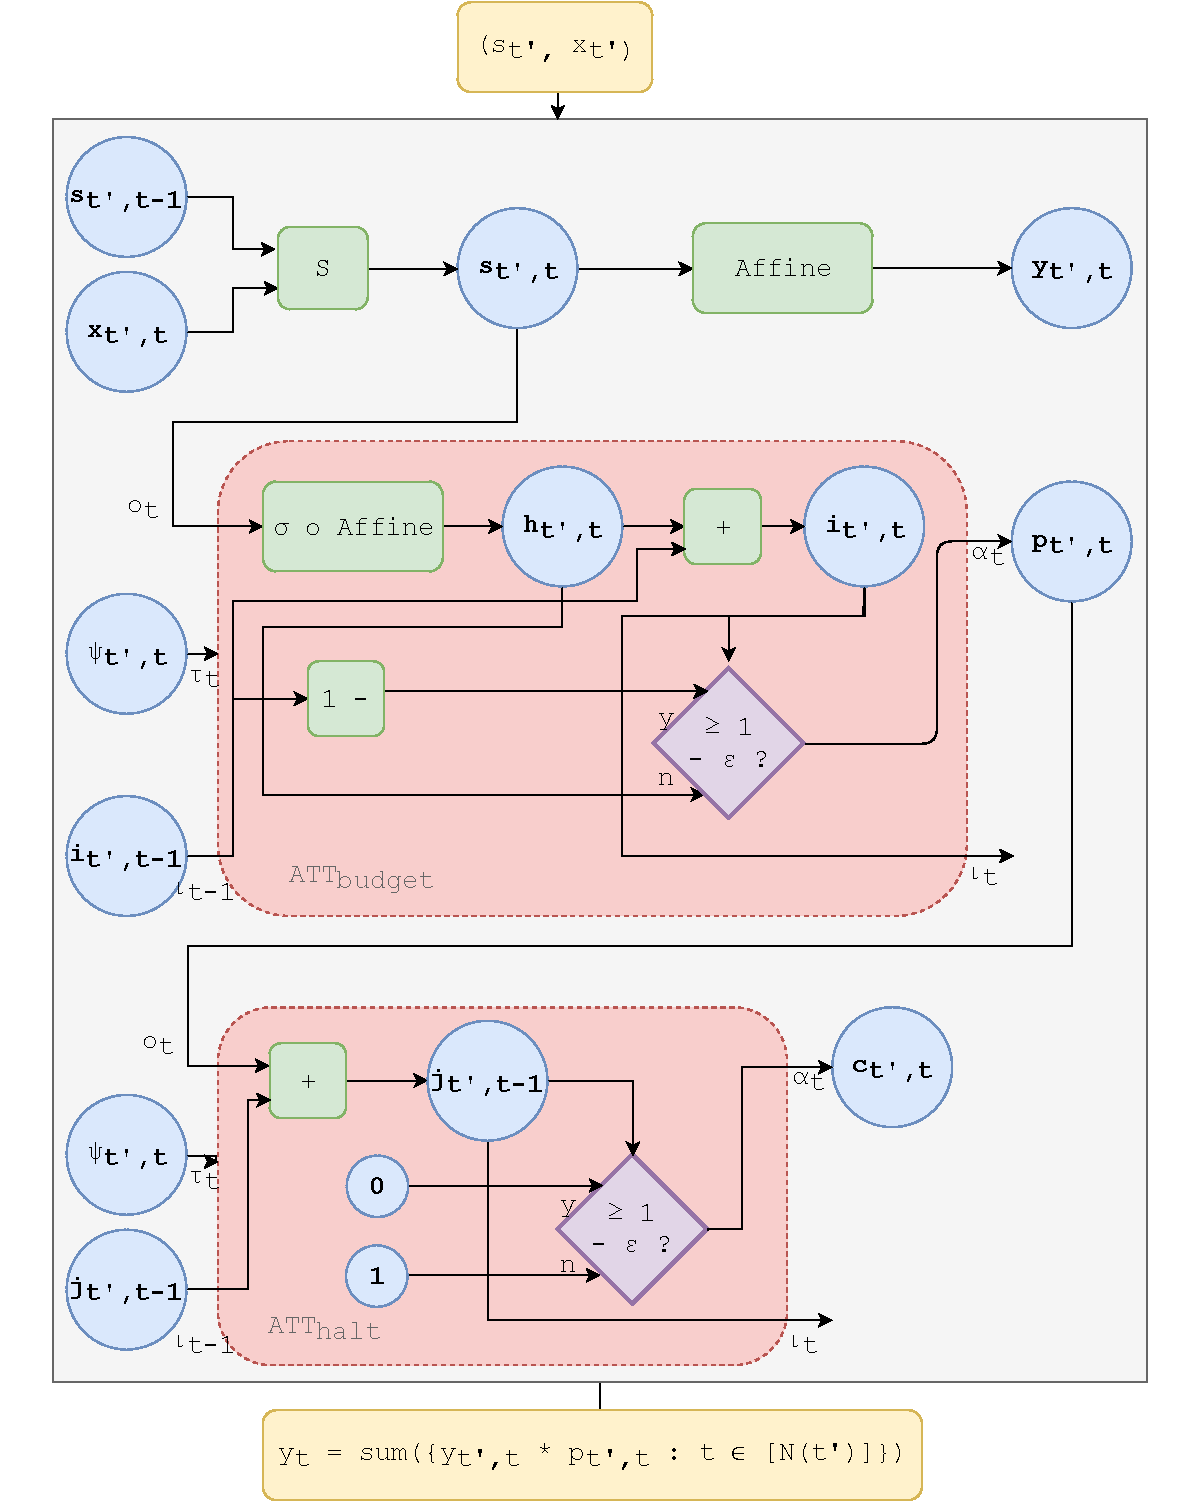
\includegraphics[width=0.6\linewidth]{./img/act.pdf}
    \label{fig:act}
    \caption{Model proposed for image captioning in~\cite{ref:act} with attentional module.}
\end{figure}

Figure~\ref{fig:act} illustrates the model proposed in the work.
The proposed model can be thought as having two attention modules:
\begin{itemize}
    \item \textbf{$ATT_{budget}$}, which computes the value $0 \le p_{t',t} \le 1$ to be spent at a given sub-step.
        In this analogy, $s_{t',t}$ -- the state of the RNN cell -- is the \emph{outer state} $o_t$;
        $\psi_t$ -- a dummy element representing the current computation sub-step -- is the \emph{target} $\tau_t$;
        and $i_{t',t}$ is the \emph{inner state}.
        The \emph{focus output} $p_{t',t}$, besides representing values to be consumed from the budget,
        can be thought of as an importance weight for the final output $y_t$, since the produced values are used to computed
        the weighted average.
    \item \textbf{$ATT_{halt}$}, which computes the value $c_{t',t} \in \{0, 1\}$, which is $1$ if the cell should continue
        further sub-steps and $0$ otherwise.
        In this analogy, $p_{t',t}$ is the \emph{outer state} $o_t$;
        $\psi_t$ -- a dummy element representing the current computation sub-step -- is the \emph{target} $\tau_t$;
        and $j_{t',t}$ is the \emph{inner state}.
\end{itemize}

It is interesting to note that an effect that emerges from these two blocks is that
\emph{the model can allocate resources to processes} both by
\emph{choosing the data to use} (in the computation of each $y_t$ weighted by a focus output)
and \emph{choosing the amount of computation time to use}.

\subsection{Recurrent Attention Model of Visual Attention}
The work~\cite{ref:ram} proposes a general recurrent model that uses visual attention at each step
by selecting a ``retina-like'' representation of a portion of the input image to carry out further computations.
At each time step $t$, the model uses the selected location $l_{t-1}$ to extract a retina-like representation
from input image.
An arbitrary action $a_t$ can be executed to possibly alter the environment.

\begin{figure}[H]
    \centering
    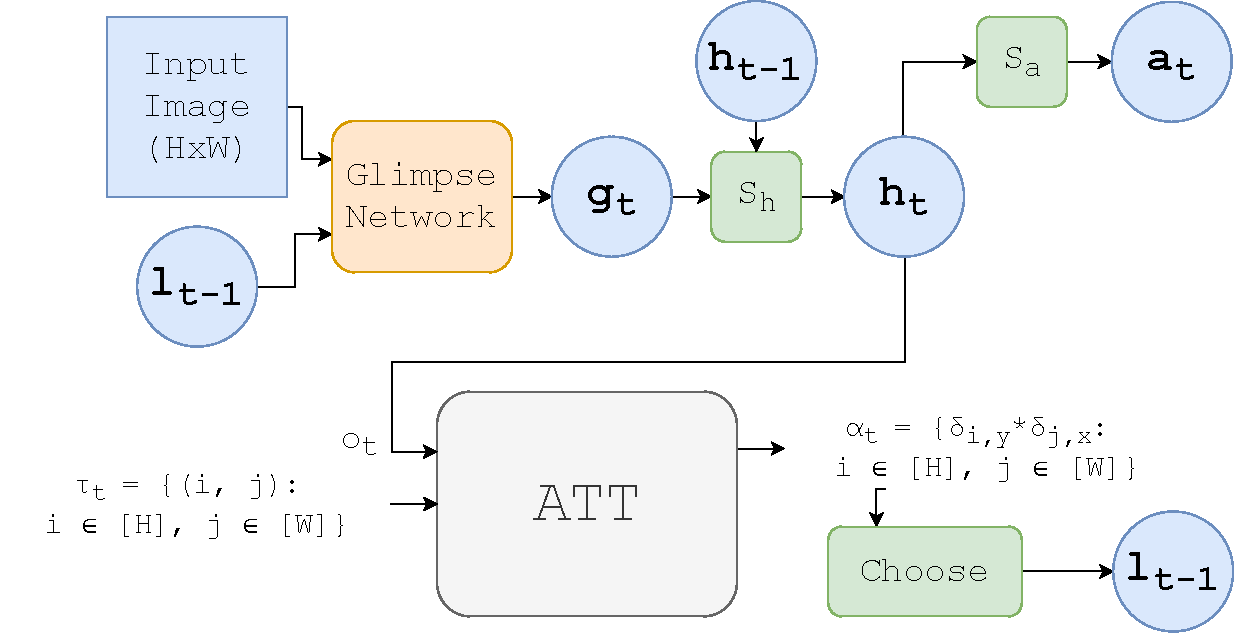
\includegraphics[width=0.6\linewidth]{./img/ram.pdf}
    \label{fig:ram}
    \caption{General recurrent architecture proposed in~\cite{ref:ram} with attentional module.}
\end{figure}

Figure~\ref{fig:ram} illustrates the model proposed in the work.
In this representation, the hidden state of the RNN $h_t$ is the \emph{outer state} input $o_t$;
The set of possible pixel coordinates $\{(i, j): i \in [H], j \in [W]\}$ (with $H, W$ as the height, width of the image)
is the \emph{focus targets} input $\tau_t$;
and the set $\{\delta_{i, y}\delta_{j, x}: i \in [H], j \in [W]\}$ is the \emph{focus output}.
Note that only the element $\delta_{i, y}\delta_{j,x}$ -- which is respective to the chosen pixel coordinates $(x, y)$
is equal to $1$.


\printbibliography
%\end{multicols}

\end{document}
